\section{Performance and Bechmarking}
\label{Chapter:Performance}

\subsection{Characterization}
An important aspect of fabricating a new technique is measuring how well it performs in different usage scenarios. The problem is, in terms of arts, not every mistake the technique makes can be regarded as an issue. Developing a metrics for judging the artistic quality of a calligraphy specimen produced by the Bezier or rotating Bezier splines is altogether a separate discussion and out of scope of this research. However, there are some aspects that we have tried to measure that give us some idea how effective the rotating Bezier splines can be.

\subsection{Supported Scripts}
By ``supported scripts'' one may imply deriving a mathematical model for a particular font or a scipt family. The mainline scripts used in calligraphy are not necessarily as mathematical as the model of the rotating Bezier splines. Especially, when the artists start to utilize their writing tool in unique ways to extract some unique value from the scripts they create, forming a mathematical model becomes practically impossible. However, since in the first place, it would be an artist who will be creating and tracing scripts on the screen of a computer, it is safe to claim that given the similarity of the emulation, rotating Bezier splines can be used to produce any script that is written with broad edge tools. However, these are some limitations inherited by this statement:

\begin{itemize}
\item If the tool changes thickness during a stroke (like a flexible brush), the best alternate to achieve a similar appearance of the script would be to use multiple splines with multiple thicknesses that overlap each other in a gradual manner.
\item Although the rotating splines have a defined tool width, we still assume the tool to be infinitely thin on the other side, more like a narrow line. This makes negligible but still some difference when the virtual tool is replaced with an actual tool. One way to overcome this issue would to come up with another rendering algorithm that also asks for this missing information. This has been discussed in later chapters when we suggest some other improvements in the overall project.
\end{itemize}

\subsubsection{Coverage}
To benchmark the performance and accuracy  of rotating bezier splines, some test results are presented here. These values are produced by comparing high resolution binary images of actual scripts, extracted with Adobe Photoshop and rasterized images produced by the twisting bezier splines produced by tracing the processed images. One-to-one pixel comparison was made using computer scripts to measure the fraction of ink that maps exactly on the original script, lies outside it or is completely missing. Table \ref{Table:Accuracy} presents some values that give some idea of efficacy of the proposed bezier splines.
\begin{table}[ht]
\centering
\resizebox{\textwidth}{!}{\begin{tabular}{| p{0.35\linewidth} | p{0.6\linewidth} |}
  \hline
\textbf{Metrics} & \textbf{Results} \\
  \hline
Percentage of area outside the original bounds & Less than 2\% \\
  \hline
Percentage of area covered&Better than $94\%$ \\
  \hline
Maximum lateral deviation of the Bezier path from the pitch line & N.A. (This list was planned in the synopsis but is no longer valid given the nature of fabricated splines.) \\
  \hline
Total number of compatible scripts & Broad edge scripts of all languages \\
  \hline
Total number of splines measured & $>100$ \\
  \hline
Total pixels compared & $9.9$~million \\
  \hline
Tested scripts & Nastaleeq, Thuluth \\
  \hline
\end{tabular}}
\caption{Benchmark of the mathematical accuracy of the twisting bezier spline curves}
\label{Table:Accuracy}
\end{table}

This metrics is comprehensive but still not complete. Some additional metrices are still needed to give a verdict about how good the proposed solution is and it is now up to the community to evolve these curves according to the needs. Table \ref{Table:AdvancedMetrices} presents a couple of those metrices that may also be desired by the researchers.

\begin{table}[ht]
\centering
\resizebox{\textwidth}{!}{\begin{tabular}{| p{0.35\linewidth} | p{0.6\linewidth} |}
  \hline
  \textbf{Metrics} & \textbf{How can it be measured} \\
  \hline
Easy of usage & A survey based on Likert scale \\
  \hline
Time efficiency of tracing an existing specimen. & Comparison of the time taken by the same artists tracing with conventional and rotating Bezier splines \\
  \hline
The artistic quality of the specimens produces. & A survey based on Likert scale and filled by a wide range of artists \\
  \hline
\end{tabular}}
\caption{Advanced metrices to gauge the effectiveness of twisting bezier splines.}
\label{Table:AdvancedMetrices}
\end{table}

Please note that the third metrics in Table \ref{Table:AdvancedMetrices} seems potent for gauging the performance of atypical supline but is no longer valid given the nature of fabricated splines.

\subsubsection{Sample Results}
As a test and a tribute, two scripts by the famous teacher, artist and author of $18$ calligraphy books, late Khursheed Gohar Qalam \cite{bib23} of the National College of Arts (NCA) were borrowed; one in Nastaleeq and other in Thuluth. Figure \ref{Fig:InkComparison} shows a detailed comparison of a part of a famous script produced by Gohar with the version traced with twisting bezier splines. The comparison unveils how accurately the bezier splines appear to be tracing the original script. The original appearing in Figure \ref{Fig:InkComparison}(a) image is first processed to be used with the spline editor and then converted to a binary image which is shown in Figure \ref{Fig:InkComparison}(b). Figure appearing in Figure \ref{Fig:InkComparison}(c), (d) and (e) are then produced by rasterizing the traced spline and a one-to-one pixel comparison of both images. See Table \ref{Table:AdvancedMetrices} which shows a quantitative measure of the trace accuracy. With these values, it is fair to assert that the twisting splines are very accurately mimicking the original sample.

However no matter how accurate they look, it must also be noted that since the original image is not available in a sufficiently high digital resolution, strictly speaking, Figure \ref{Fig:InkComparison}(d) and (e) do not do not show the true picture of the error that the curves produce but only a reasonably good estimate. The final verdict about the accuracy can only be given in form of the appeal this technique gets when actually presented in the community.

Figure \ref{Fig:Nastaleeq} and \ref{Fig:Thuluth} show sample outputs produced by tracing two of famous Gohar's articles in ``Nastaleeq'' and ``Thuluth'' scripts. The twisting splines do contain vector data and have no resolution but for the sake of presentation, the images have been rasterized by ``Gregor''.
\begin{figure}
  \centering
  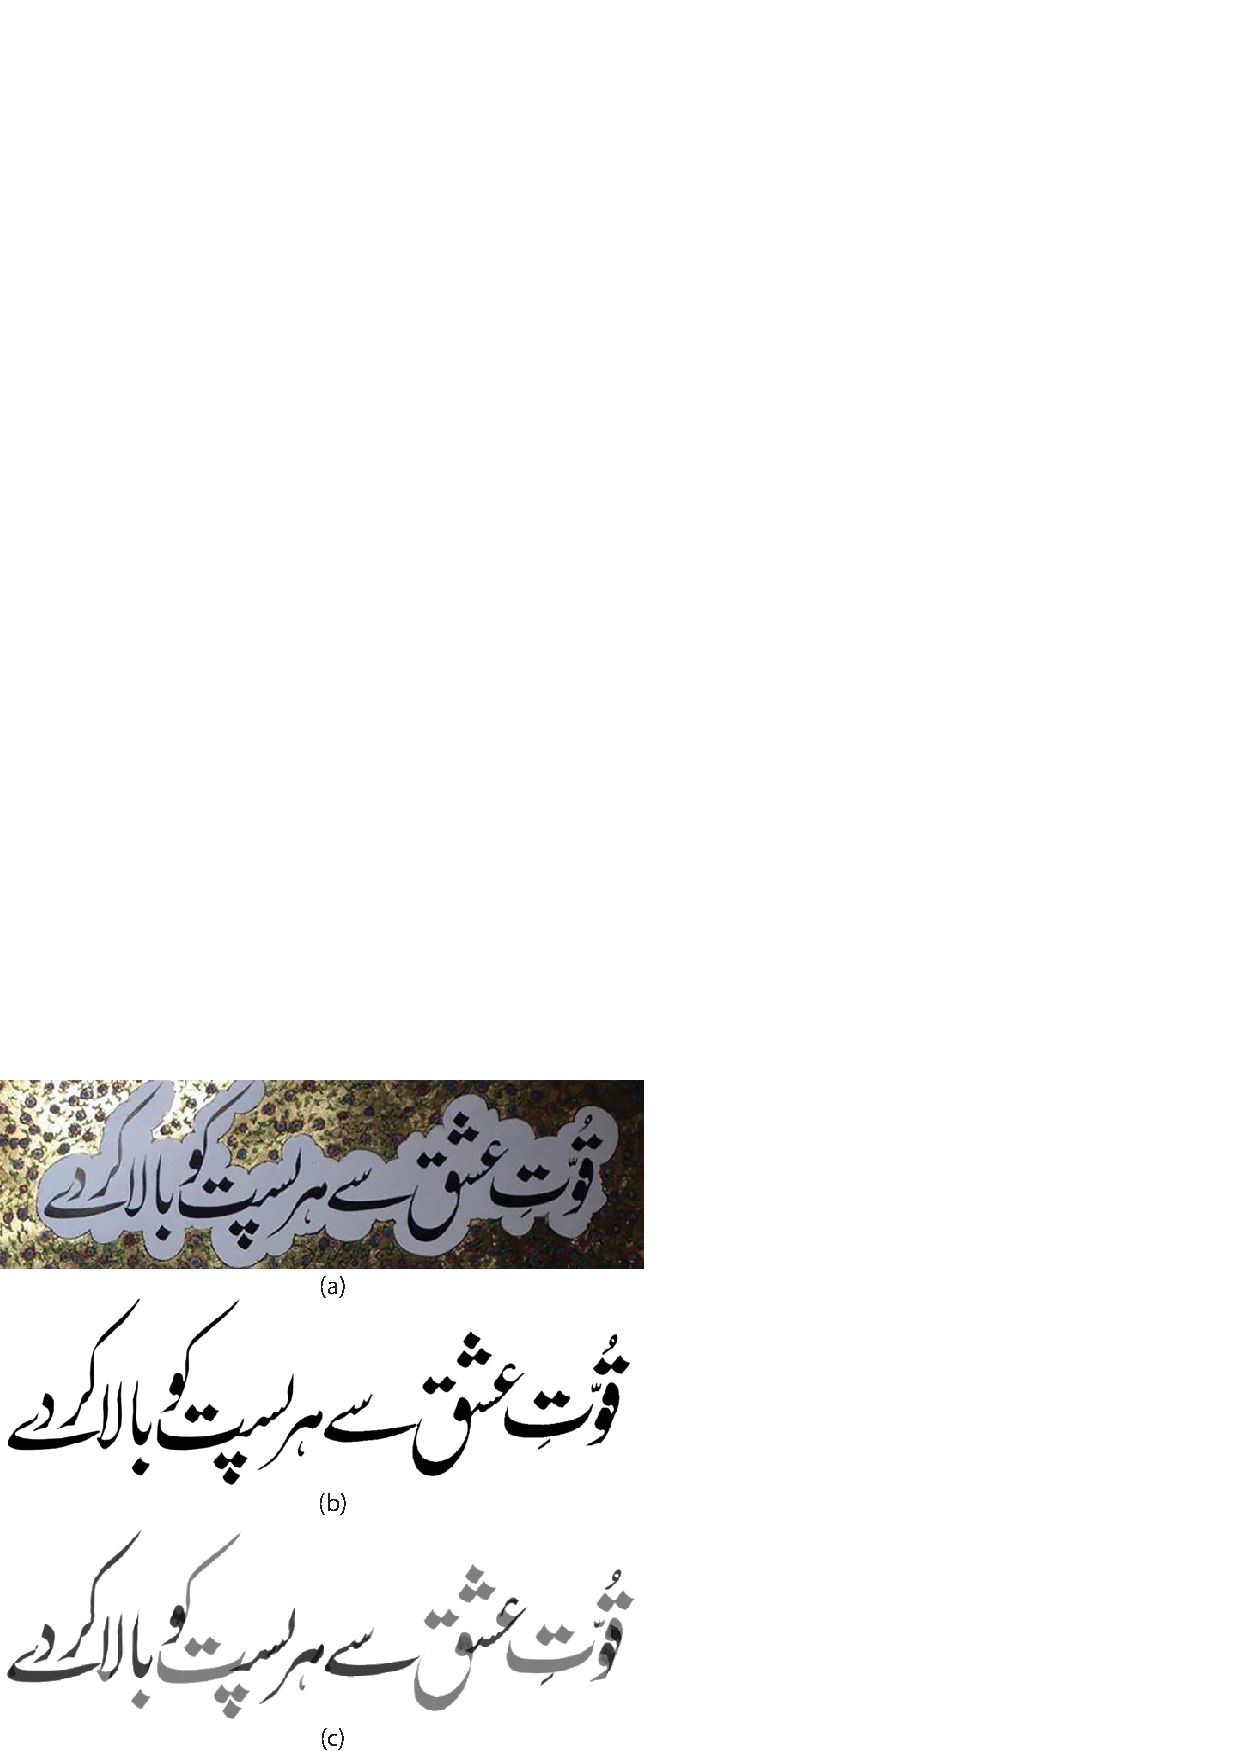
\includegraphics[width=0.6\textwidth]{../Images/NastaleeqSample.pdf}
  \caption{A specimen produced in ``Nastaleeq'' script. (a) Original photograph of the specimen (b) Rasterized binary image of the twisting spline curves. (c) Rasteriezd shaded image of the twisting spline curves highlighting individual curve parts.}
  \label{Fig:Nastaleeq}
\end{figure}

\begin{figure}
  \centering
  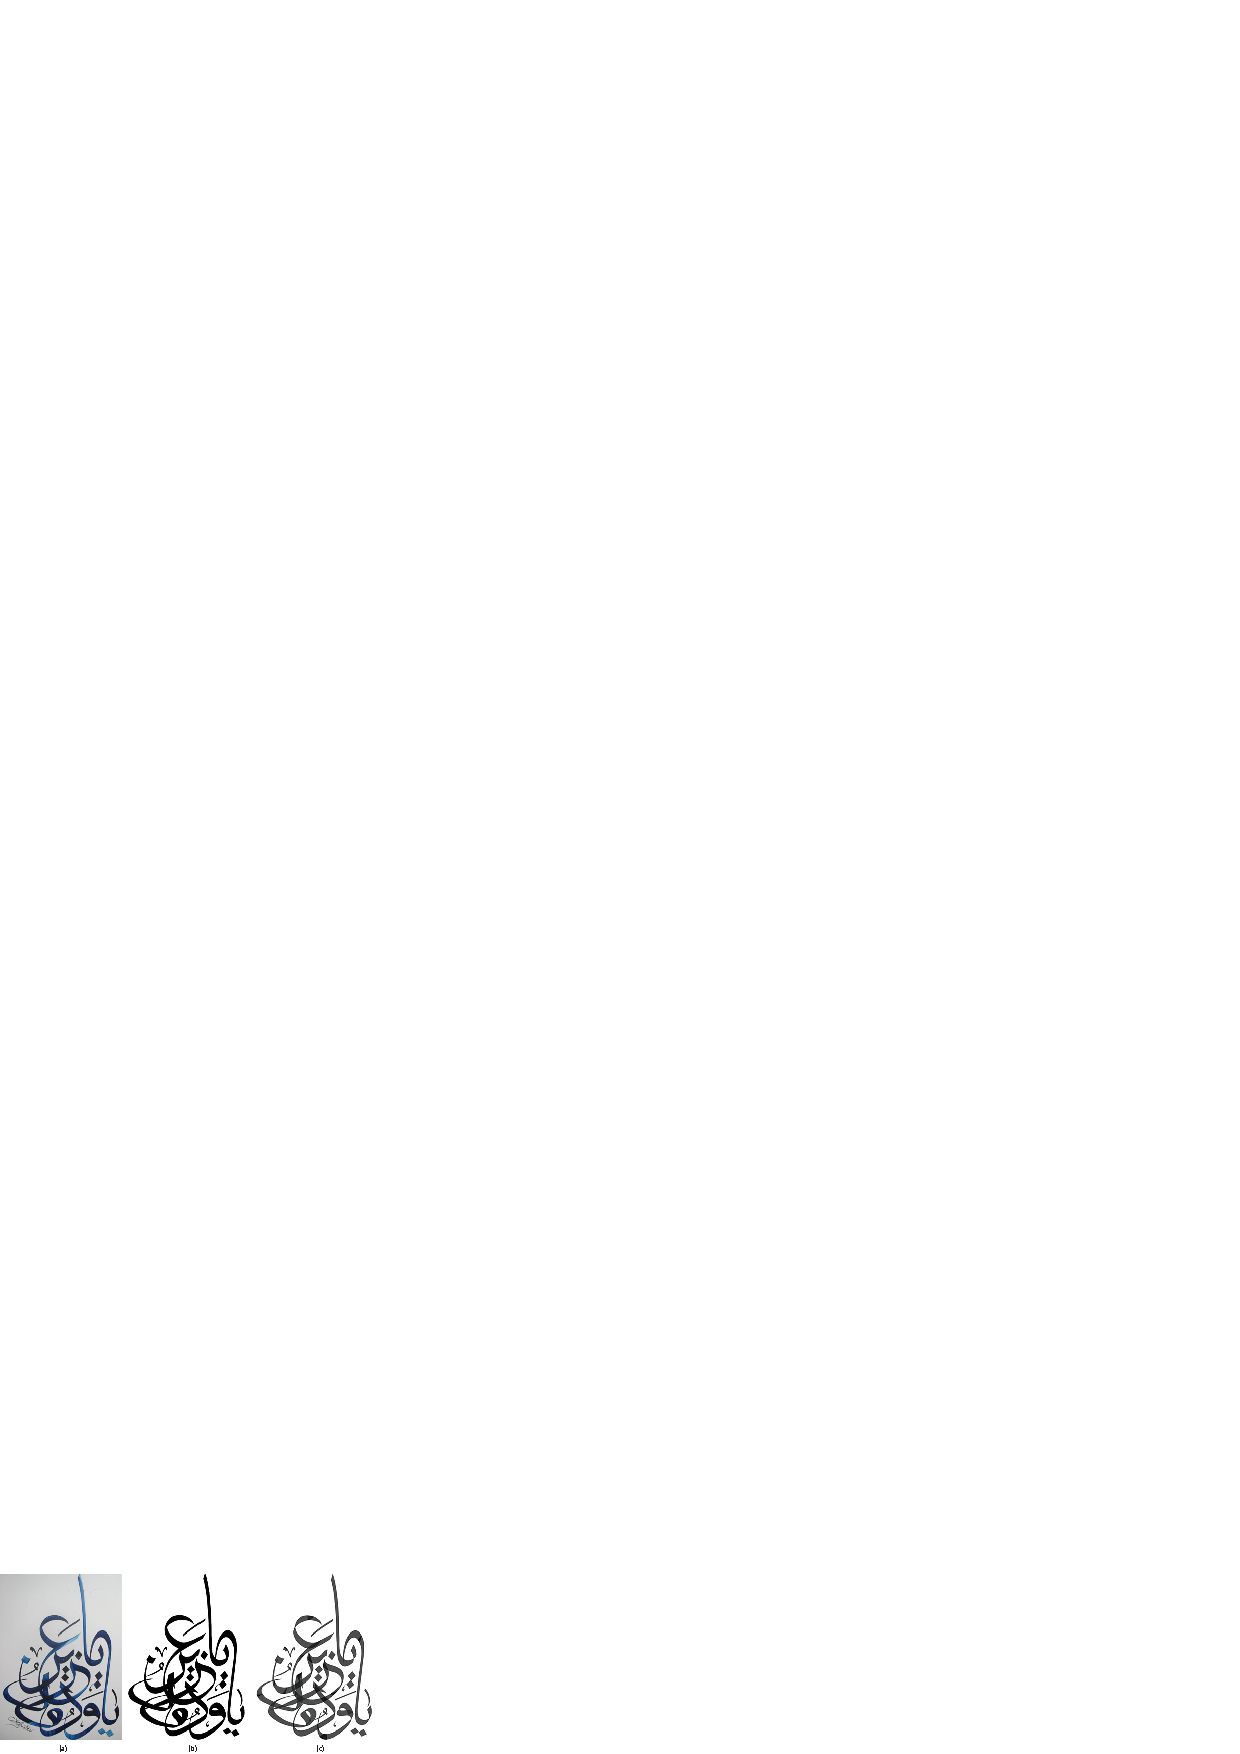
\includegraphics[width=1\textwidth]{../Images/ThuluthSample.pdf}
  \caption{A specimen produced in ``Thuluth'' script. (a) Original photograph of the specimen (b) Rasterized binary image of the twisting spline curves. (c) Rasteriezd shaded image of the twisting spline curves highlighting individual curve parts.
  }
  \label{Fig:Thuluth}
\end{figure}

\subsubsection{Machine Data Generation and Simulation}
    To check how accurately the data generated by these splines can be traced by an actual robotic manipulator, computer simulation was used. We use an open-source simulator, developed in-house for the task. The simulator can simulate a $6$~DoF robotic manipulator with on-screen $3$D visualization.
    
    Using the same model of the spline model, the simulator first rasterizes the whole spline and then transforms the two dimensional points onto a plannar surface simulated on a user desired position in the workspace. Then it creates a pseudo machine code to mimic the tool changes required before each stroke and the transformed rasterized points are directly considered as G-Codes for the manipulator. Once computed it starts implementing the program.

    For the sake of analysis, in parallel, the end effector orientation is captured continuously to construct an ink mark with each sweep of the tool. The reproduced image is then used for analysis. The results of such a comparison can be seen in Table \ref{Table:MachineDataMetrices}. The value indicate that the robot very closely reproduces the given spline thus verifying the thesis of the research.

    \begin{table}[ht]
    \centering
    \resizebox{\textwidth}{!}{\begin{tabular}{| p{0.3\linewidth} | p{0.3\linewidth} |  p{0.2\linewidth} |  p{0.2\linewidth} |}
      \hline
      & \textbf{Reference} & \textbf{Coverage} & \textbf{Extra} \\
      \hline
      \multicolumn{4}{|l|}{\textbf{Nastaleeq}}\\
      \hline
      Rotating Bazier Spline & Original Image & 95.8\% & 5.4\% \\
      \hline
      Machined Output & Original Image & 96.7\% & 7.0\% \\
      \hline
      Machined Output & Rasterized Image & 96.7\% & 4.3\% \\
      \hline
      \multicolumn{4}{|l|}{\textbf{Thuluth}}\\
      \hline
      Rotating Bazier Spline & Original Image & 93.4\% & 2.8\% \\
      \hline
      Machined Output & Original Image & 95.0\% & 3.4\% \\
      \hline
      Machined Output & Rasterized Image & 97.8\% & 4.4\% \\
      \hline
    \end{tabular}}
    \caption{Benchmark of the mathematical accuracy of the twisting bezier spline curves with a simulated manipulator}
    \label{Table:MachineDataMetrices}
    \end{table}
\clearpage        